\newpage
\chapter{MIDAS}
\label{chap:mc}
\workTodo{In diesem Kapitel werden grundlegende Themen behandelt, die im Rahmen des Forschungsprojekts zum Verständnis der Ausreißer-Erkennung in Graphen gedient haben.}
\workTodo{Related Work: Sedanspot, RHSS}

Erst erklären wie der MIDAS funktioniert. Und zum Laufen gebracht mit Graphen über die Zeit ENRON \& DARPA. Im Anschluss auf Zeitreihendaten angewendet.


\section{Grundlagen}
\label{sec:mc-gl}
\workTodo{Einführung in den Algorithmus, NodeHash- sowie EdgeHash-Funktionen beschreiben}

MIDAS, Eng. \textit{Microcluster-Based Detector of Anomalies in Edge Streams}, steht für einen Algorithmus, der plötzlich auftretende Ausbrüche von Aktivitäten in einem Netzwerk bzw. Graphen erkennt. Dieses vermehrte Auftreten von Aktivitäten zeigt sich durch viele sich wiederholende Knoten- und Kantenpaare in einem sich zeitlich entwickelnden Graphen, die Mikrocluster bezeichnet werden. Mikrocluster bestehen demnach aus einem vermehrten Vorkommen eines einzigen Quell- und Zielpaares bzw. einer Kante $(u,v)$  \workTodo{Folgender Absatz kann vor der Beschreibung des Algorithmus eingefügt werden, wie im Paper auch} Dies geschieht in Echtzeit, wobei jede Kante in konstanter Zeit und Speicher verarbeitet wird. In der Theorie garantiert er eine False-positive-Wahrscheinlichkeit und ist durch einen 162 bis 644 mal schnelleren Ansatz, sowie einer 42\% bis 48\% höhere Genauigkeit, im Hinblick auf die AUC, sehr effektiv. \citep[vgl.][S.~1]{MIDAS}

Anwendungsfälle für MIDAS sind die Erkennung von Anomalien in Computer-Netzwerken, wie SPAM oder DoS-Angriffe oder Anomalien in Kreditkartentransaktionen.


\subsubsection{Count-Min-Sketch}
\label{sec:mc-gl-cms}
Damit die relevanten Informationen für den Algorithmus mit einem konstanten Speicher verarbeitet werden, wird Count-Min-Sketch genutzt, dass eine Streaming-Datenstruktur mithilfe der Nutzung von Hash-Funktionen entspricht. Count-Min-Sketch zählt somit die Frequenz einer Aktivität bei Streaming-Daten. Diese Datenstruktur hat ebenfalls den Vorteil, dass man zu Beginn keine Kenntnis über die Anzahl an Quell- und Zielpaaren haben muss.

MIDAS verwendet zwei Arten von CMS. Die erste Variante $s_{uv}$ wird als die Anzahl an Kanten von $u$ zu $v$ bis zum aktuellen Zeitpunkt $t$ definiert. Durch die CMS-Datenstruktur werden alle Zählungen von $s_{uv}$ approximiert, sodass jederzeit eine annähernde Abfrage $\hat{s}_{uv}$ erhalten werden kann.
Die zweite Variante $a_{uv}$ wird als die Anzahl an Kanten  von $u$ zu $v$ im aktuellen Zeitpunkt $t$ definiert. Dieser CMS ist identisch zu $s_{uv}$, wobei bei jedem Übergang zum nächsten Zeitpunkt die Datenstruktur zurückgesetzt wird. Dadurch resultiert aus dem CMS für den aktuellen Zeitpunkt die annähernde Abfrage $\hat{a}_{uv}$. \citep[vgl.][S.~3]{MIDAS}


\workTodo{chi-squared}


\subsection{Erkennung von Mikrocluster}
\label{sec:mc-gl-dm}


\subsection{Experimente}
\label{sec:m-ex}
\workTodo{ausformulieren, bilder einfügen}
- DARPA und ENRON Datensätze
- Jumpsup Datensatz von Marcus

-DARPA AUC 91%
-ENRON identisch mit SEDANSPOT-labels außer September 2000

Schwierigkeit geeignete Datensätze zu finden, dazu gibt es ein Paper

Wenn man die Anomalyscores als gewichte nimmt, kommen Graphen in Networkx raus in denen man die anomalous nodes identifizieren kann dabei sollten es Edges sein..

\subsubsection{Einführung}
\label{sec:mc-gl-cms-in}

\workTodo{Stichworte sammeln}

\section{Ergebnisse Ausreißererkennung in Zeitreihen}
Wie in \autoref{chap:trsnsMidas} beschrieben muss die Zeitreihe zunächst in verschiedene Netzwerke umgewandelt werden. In \autoref{img:midasTSresults} ist das Ergebnis der Ausreißererkennung mit Midas abgebildet. Der Ausreißer wird von dem Algorithmus identifiziert, jedoch ist der Verlauf des Ausreißer Scores schwierig zu interpretieren. Es ist zu erkennen, das zu beginn jedes Abschnittes der Ausreißer Score sehr hoch ist und am Ende niedrig(Ausnahme Abschnitt mit Ausreißer). Grund hierfür ist, das der Algorithmus die Anzahl der Kanten in einem Abschnitt mit der Anzahl an Katen aus vorherigen Abschnitten vergleicht. Zu Beginn eines jeden Abschnitts ist die Anzahl an Kanten deutlich geringer, deshalb ist der Ausreißer Score auch höher. Am Ende eines Abschnitts ist die Anzahl an Kanten in Relation identisch, deshalb ist der Ausreißer Score höher. Der Abschnitt in welchem sich der Ausreißer befindet ist deutlich größer als die anderen Abschnitte. Der Grund hierfür ist, das die Anzahl an Kanten deutlich höher ist als in den anderen Abschnitten. Für jede Kante wird ein zusätzliches Element zum Ausreißer Score hinzugefügt. Da Kantengewichte in dem Abschnitt mit dem Ausreißer deutlich größer sind, resultiert dies in deutlich mehr Kanten. 
\label{sec:resultsOTs}

\begin{figure}[h]
	\centering
	\subfloat[Caption for sub-figure1]{
		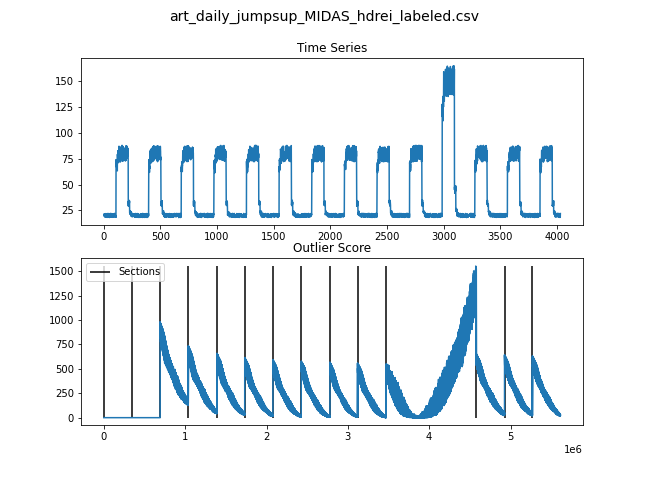
\includegraphics[width=0.5\textwidth]{fig/resultsMidasTS/art_daily_jumpsup_MIDAS_hdrei_labeled_result.png}}
	\subfloat[Caption for sub-figure1]{
		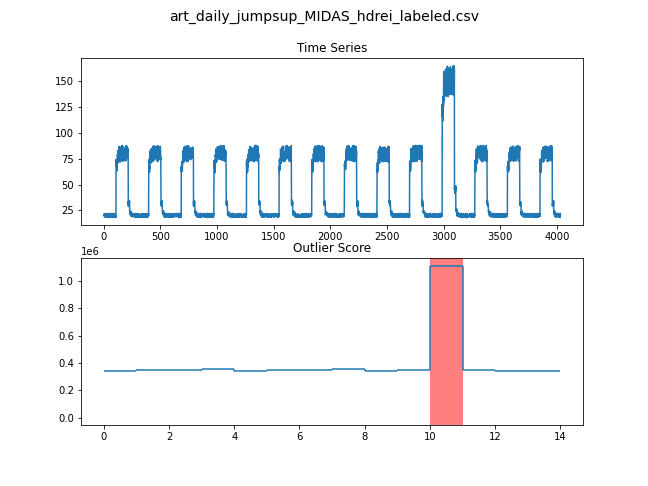
\includegraphics[width=0.5\textwidth]{fig/resultsMidasTS/result_without_midas.png}}
	\caption{Vergelich Perculation Algorithmus mit Sliding Window Verfahren und ohne Sliding Window Verfahren}
	\label{img:midasTSresults}
\end{figure}

Da der Midas Algorithmus lediglich die Anzahl an Kanten zwischen zwei Knoten zählt um Ausreißer zu erkennen, verglichen wir den Midas Algorithmus mit einem naiven Algorithmus der lediglich die Gesamtanzahl an Knoten in einem Abschnitt zählt. Es konnte festgestellt werden, dass der naive Ansatz den Midas Algorithmus mithalten kann. Aus diesem Grund wurden keinerlei weitere Datensätze untersucht. 
\workTodo{Vielleicht den Algorithmus einmal auf einzelne Peaks testen vielleicht bringt das was.}
\label{sec:resultTSwithoutMidas}

\begin{figure}[h]
	\centering
	\subfloat[Caption for sub-figure1]{
		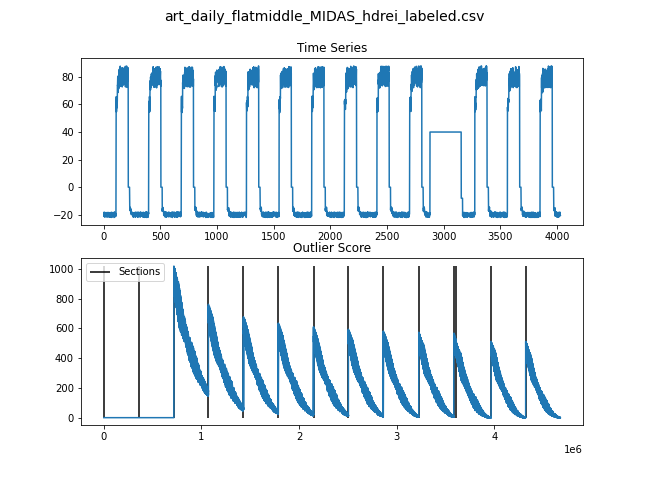
\includegraphics[width=0.5\textwidth]{fig/resultsMidasTS/art_daily_flatmiddle_MIDAS_hdrei_labeled_result.png}}
	\subfloat[Caption for sub-figure1]{
		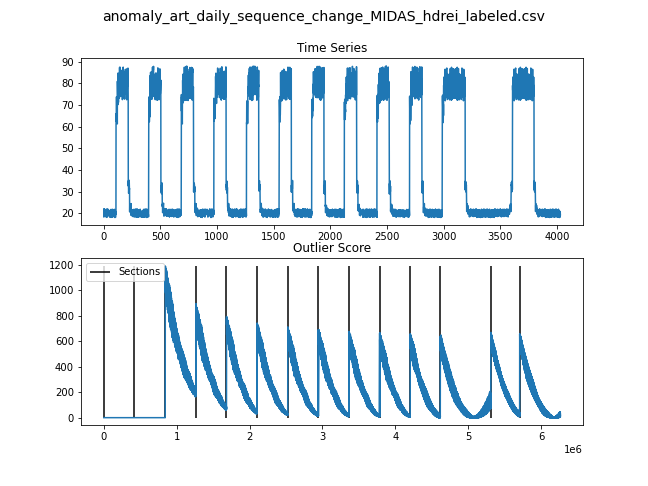
\includegraphics[width=0.5\textwidth]{fig/resultsMidasTS/anomaly_art_daily_sequence_change_MIDAS_hdrei_labeled_result.png}}
	\caption{Vergelich Perculation Algorithmus mit Sliding Window Verfahren und ohne Sliding Window Verfahren}
	\label{img:midasTSresults}
\end{figure}

Der Algorithmus funktioniert lediglich bei einem Ausschlag nach oben, weil der Ausschlag nach oben zu gro�en Gewichten innerhalb des Netzes f�hrt. Die gro�en Gewichte f�hren zu vielen Kanten in den Daten was dan zu einem Anstieg des Ausrei�er Scores f�hrt.

Bei anderen Ausrei�er Typen ist teilwei�e das genenteil der Fall, wie in 4.2a. Hier gibt es in dem Abschnitt mit dem Ausrei�er nur sehr geringe Kantengewichte. Das f�hrt sehr wenigen Kanten in den Daten. Jedoch schl�gt der Ausrei�er Score nicht stark aus. In 4.2b ist der Abschnitt ein bisschen gr��er.

\begin{figure}[h]
	\centering
	\subfloat[Caption for sub-figure1]{
		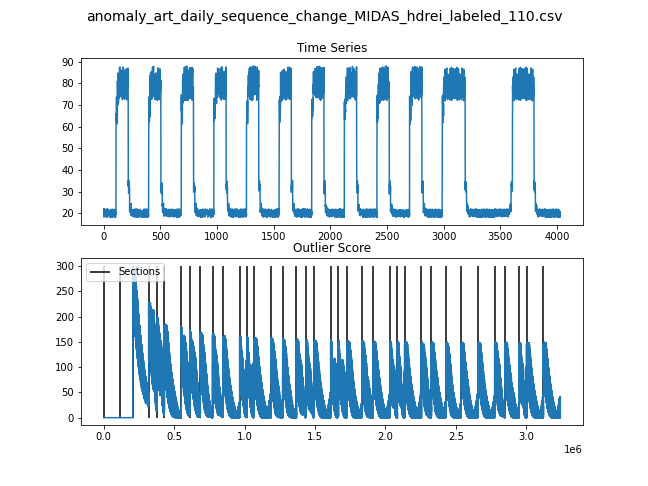
\includegraphics[width=0.5\textwidth]{fig/resultsMidasTS/anomaly_art_daily_sequence_change_MIDAS_hdrei_labeled_110_result.png}}	
	\subfloat[Caption for sub-figure1]{
		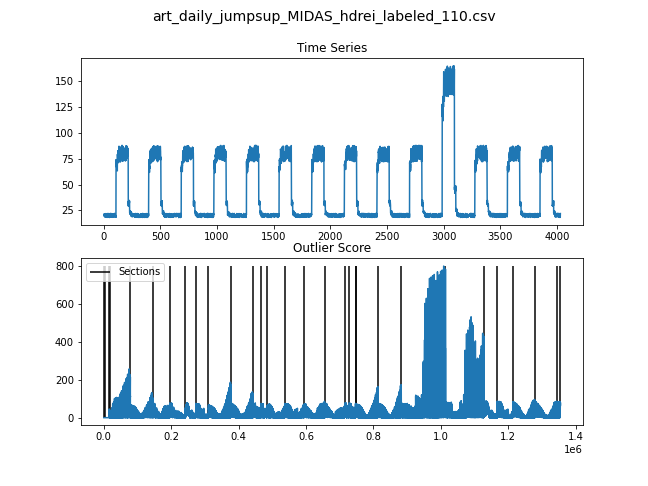
\includegraphics[width=0.5\textwidth]{fig/resultsMidasTS/art_daily_jumpsup_MIDAS_hdrei_labeled_110_result.png}}
	\caption{Vergelich Perculation Algorithmus mit Sliding Window Verfahren und ohne Sliding Window Verfahren}
	\label{img:midasTSresults}
\end{figure}


Die Ver�nderung der Fenstergr��e nutzt nur Bedingt etwas. F�r den Ausrei�er nach oben werden die ausschl�ge im Ausrei�er Score noch deutlicher. Alle anderen funktionieren weiterhin nicht.

\begin{figure}[h]
	\centering
	\subfloat[lol]{
		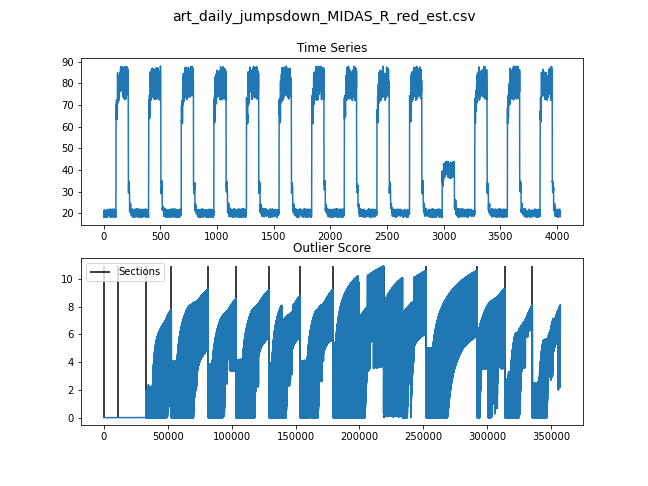
\includegraphics[width=0.5\textwidth]{fig/reultsMidasR/art_daily_jumpsdown_MIDAS_R_red_est_result}}
	\subfloat[lol]{
		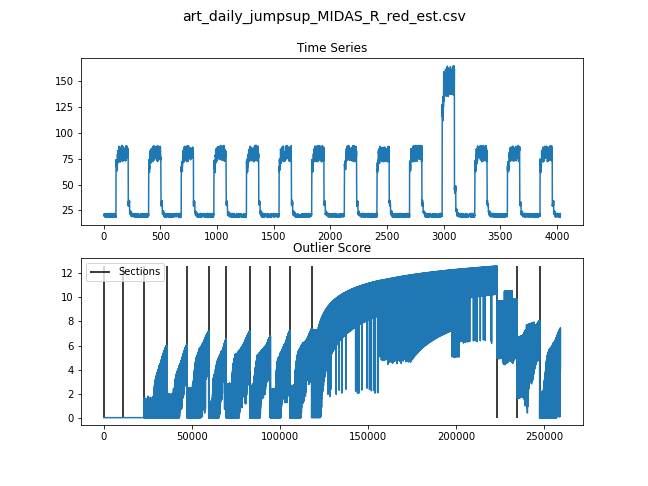
\includegraphics[width=0.5\textwidth]{fig/reultsMidasR/art_daily_jumpsup_MIDAS_R_red_est_result}}
	\caption{Vergelich Perculation Algorithmus mit Sliding Window Verfahren und ohne Sliding Window Verfahren}
	\label{img:midasTSresults}
\end{figure}

Auch der Midas R Algorithmus f�hrt nicht zu einer verbesserung der Ergebnisse. Der eine Ausrei�er wird eriterhin erkannt. Alle anderen Ausrei�er Typen werden nicht erkannt. 

